% !TeX spellcheck = da_DK
\documentclass[11pt,a4paper,oneside]{article}

% Overordnet opsætning
\setlength\parindent{24pt}
\setlength\parskip{3pt}
\setlength{\headheight}{14pt}
\renewcommand{\baselinestretch}{1.5}

\usepackage[utf8]{inputenc}
\usepackage[danish,english]{babel}
\usepackage{amsfonts,amsmath} %math: align og gather mm.; fonts: flere forskellige symboler
\usepackage[left=2cm, right=2cm, bottom=2cm]{geometry}
\usepackage{enumitem} %anvendes til ændring i itemize mm.
\usepackage{fancyhdr} %Opsaening af sidehoved og -fod
\usepackage{lastpage} % Side "x af X".
\usepackage[ocgcolorlinks,linkcolor=black,urlcolor=black]{hyperref}
\usepackage{indentfirst} %"Indent" efter section og chapters etc.
\usepackage{graphicx} % for plotting graphs in matrix
\usepackage{subcaption} % figure "footnotes"

% bibliography
% \usepackage{csquotes}
% \usepackage{biblatex}
% \addbibresource{bibliography.bib}

% Ændring af titler
\usepackage{sectsty}
\subsectionfont{\normalfont\bfseries}
\subsubsectionfont{\normalfont\itshape\underline}

%Rstudio pakker
\usepackage[svgnames]{xcolor}
\usepackage{listings}

\lstset{language=R,
    basicstyle=\small\ttfamily,
    stringstyle=\color{DarkGreen},
    otherkeywords={0,1,2,3,4,5,6,7,8,9},
    morekeywords={TRUE,FALSE},
    deletekeywords={data,frame,length,as,character},
    keywordstyle=\color{blue},
    commentstyle=\color{DarkGreen},
}

% fancy table
\usepackage{booktabs}
\usepackage{multirow}

\pagestyle{fancy}
\fancyhf{}
\fancyhead[L]{\leftmark}
\fancyhead[R]{\rightmark}
\lfoot{\author}
\rfoot{\thepage}
\renewcommand{\headrulewidth}{0.4pt}
\renewcommand{\footrulewidth}{0.4pt}

%Table of Contents (toc) 
\setcounter{secnumdepth}{0}
\setcounter{tocdepth}{1}

%symbolforkortelser
\newcommand{\lll}{\mathcal{L}}
\newcommand{\LL}{\Leftrightarrow}
\newcommand{\lp}{\left(}
\newcommand{\rp}{\right)}
\newcommand{\rb}{\right]}
\newcommand{\lb}{\left[}
\newcommand{\lc}{\left\{}
\newcommand{\rc}{\right\}}
\newcommand{\dd}{\mathrm{d}}
\newcommand{\cc}{\mathbb{C}}
\newcommand{\ee}{\mathbf{E}}
\newcommand{\ff}{\mathcal{F}}
\newcommand{\for}{\text{ for }}
\newcommand{\ggg}{\mathcal{G}}
\newcommand{\hh}{\mathcal{H}}
\newcommand{\pp}{\mathcal{P}}
\newcommand{\qq}{\mathcal{Q}}
\newcommand{\vv}{\mathbf{V}}
\newcommand{\rr}{\mathbf{R}}
\newcommand{\nn}{\mathbf{N}}
\newcommand{\nnn}{\mathcal{N}}
\newcommand{\ii}{\mathbf{1}}
\newcommand{\iid}{\overset{iid}{\sim}}
\newcommand{\bs}{\text{BS}}
\newcommand{\sumn}{\sum_{i=1}^n}
\newcommand{\sumt}{\sum_{t=1}^T}
\newcommand{\var}{\text{VaR}_{t,1}^\alpha}
\DeclareMathOperator*{\argmin}{\arg\,\min}


\selectlanguage{english}

% Sidetal er romertal frem til første kapitel
\pagenumbering{roman}

\lstset{language=R}

% Environment for theorems etc.
\newtheorem{theorem}{Theorem}
\newtheorem{corollary}{Corollary}[theorem]
\newtheorem{lemma}[theorem]{Lemma}
\newtheorem{assumption}{Assumption}
\newtheorem{proof}{Proof}

\title{Exercise sheet 9}
\author{William Gram}
\date{\today}

\begin{document}
\maketitle

\pagenumbering{arabic}
\rfoot{\thepage}
\lfoot{Code at (click): \href{https://github.com/WiGram/fe_python}{GitHub/WiGram}}

\section{Exercise 1: EM Algorithm}
\renewcommand{\theequation}{1.\arabic{equation}}
\setcounter{equation}{0}

Here we consider the two-state mixture volatility model, given by:
\begin{align*}
    x_t 
        &= \sigma_t z_t, \quad z_t \iid \nnn\lp 0, 1\rp \\
    \sigma_t^2
        &= \begin{cases}
                \sigma_1^2, & s_t = 1,\\
                \sigma_2^2, & s_t = 2
            \end{cases},
\end{align*}

where $s_t \sim i.i.d.$ with probabilities $\pp\lp s_t = 1\rp = p = 1 - \pp\lp s_t = 2\rp$. Generally, it is assumed, that we observe the log-return sequence $x_t$ but not the state sequence $s_t$.

\subsection{1.1}
In the case where both sequences $x_t$ and $s_t$ are observed for all $t$, we are asked to say how we would estimate the model parameters $p$ and $\sigma_1^2, \sigma_2^2$.

Since we can observe $s_t$ we know if $\ii_{\lc s_t = 1\rc} = \ii_t^1 = 1$ holds. Thus:
\begin{align}
    \hat p = \frac{\sumt \ii_t^1}{T}.
\end{align}

The volatility $\sigma_1^2$ is then the average of the volatilities in the periods where $\ii_t = 1$, i.e.:
\begin{align}
    \hat \sigma_i^2 = \frac{\sumt x_t^2 \ii_t^i}{\sumt \ii_t^i}, \quad i = 1, 2.
\end{align}

\subsection{1.2}
Next, we denote the joint density function of $x_t$ and $s_t$ by $f\lp x_t, s_t\rp$. With abuse of notation, we also define $x_{1:T} = x_1, \dots, x_T$ and $s_{1:T} = s_t, \dots, s_T$.

We are then asked to show, that the likelihood function, conditional on the first observation, is given by:
\begin{align}
    \lll_T\lp \theta\rp = \lll\lp x_{1:T}, s_{1:T}; \theta\rp = \prod_{t=2}^T f\lp x_t\vert s_t\rp p\lp s_t\rp.
\end{align}

Before we start, we note that
\begin{align}
x_t \vert x_{1:t}, s_{1:t} \overset{d}{=} x_t \vert s_t, \quad  s_t \vert x_{1:t}, s_{1:t} \overset{d}{=} s_t.
\end{align}

That is, there is no historical dependence between the model variables, and $s_t$ influences only the contemporary $x_t$ and is influenced by nothing itself.

Thus, we have that:
\begin{align}
    f\lp x_{1:T}, s_{1:T} \rp 
        &= f\lp x_T \vert x_{1:T-1}, s_{1:T} \rp f\lp x_{1:T-1}, s_{1:T}\rp \notag \\
        &= f\lp x_T \vert x_{1:T-1}, s_{1:T} \rp f\lp s_T\vert s_{1:T-1}, x_{1:T-1} \rp f\lp s_{1:T-1}, x_{1:T-1}\rp.
\end{align}

From (1.4) we see that we have $f\lp x_{1:T}, s_{1:T}\rp$ on the LHS and $f\lp x_{1:T-1}, s_{1:T-1}\rp$ on the RHS. Thus, when we have reduced the conditional density functions in (1.5) we can simply repeat.

From (1.4) we have that (1.5) can be rewritten as:
\begin{align}
    f\lp x_{1:T}, s_{1:T} \rp 
        &= f\lp x_T \vert x_{1:T-1}, s_{1:T} \rp f\lp s_T\vert s_{1:T-1}, x_{1:T-1} \rp f\lp s_{1:T-1}, x_{1:T-1}\rp \notag \\
        &= f\lp x_T \vert s_T \rp f\lp s_T \rp f\lp s_{1:T-1}, x_{1:T-1}\rp \notag \\
        &= f\lp x_T \vert s_T \rp p\lp s_T\rp f\lp s_{1:T-1}, x_{1:T-1}\rp,
\end{align}

where the last equality in (1.6) derives from the pdf of $s_t$ being the probability mass function, $s_t$ being discrete.

By deduction, we note that:
\begin{align}
    f\lp x_{1:T}, s_{1:T} \rp 
        &= f\lp x_T \vert s_T \rp p\lp s_T\rp  f\lp x_{T-1} \vert s_{T-1} \rp p\lp s_{T-1}\rp f\lp s_{1:T-2}, x_{1:T-2}\rp \notag \\
        &= \Pi_{t=T-1}^T  f\lp x_t \vert s_t \rp p\lp s_t\rp f\lp s_{1:T-2}, x_{1:T-2}\rp.
\end{align}

This can of course further be factorised, to attain:
\begin{align}
    f\lp x_{1:T}, s_{1:T} \rp 
        = \Pi_{t=T-(T-2)}^T  f\lp x_t \vert s_t \rp p\lp s_t\rp f\lp s_{1:T - (T-1)}, x_{1:T - (T-1)}\rp 
        = f\lp s_1, x_1\rp \Pi_{t=2}^T  f\lp x_t \vert s_t \rp p\lp s_t\rp.
\end{align}

Neglecting the known term $f\lp s_1, x_1\rp$ we have that:
\begin{align}
    \lll_T\lp \theta\rp = \Pi_{t=2}^T  f\lp x_t \vert s_t \rp p\lp s_t\rp,
\end{align}
which is what we wanted to show.

\subsection{1.3}
We now consider $\lll$ from question (1.2), taking $\log$ thereof and thus deriving the log-likelihood:
\begin{align}
    \ell_T\lp \theta\rp = \log\lp \lll_T\lp \theta\rp\rp = \log\lc \Pi_{t=2}^T  f\lp x_t \vert s_t \rp p\lp s_t\rp\rc.
\end{align}

Next, because we can observe $s_t$, for each $t$ we know what $f\lp x_t \vert s_t\rp p\lp s_t\rp$ is. That is, we have that:
\begin{align}
    f\lp x_t \vert s_t\rp p\lp s_t\rp
        =
        \begin{cases}
            f\lp x_t \vert s_t = 1\rp p, & s_t = 1,\\
            f\lp x_t \vert s_t = 2\rp \lp 1 - p\rp, & s_t = 2
        \end{cases}.
\end{align}

Equation (1.11) can be rewritten as:
\begin{align}
    f\lp x_t \vert s_t\rp p\lp s_t\rp
        = \lp f\lp x_t \vert s_t = 1\rp p \rp^{\ii_t^1}
        \lp f\lp x_t \vert s_t = 2\rp \lp 1 - p \rp \rp^{\ii_t^2} = \lp f_1 \lp x_t\rp p\rp^{\ii_t^1}\lp f_2\lp x_t\rp \lp 1 - p\rp\rp^{\ii_t^2}.
\end{align}

Consequently, combining (1.12) with (1.10) we have that:
\begin{align}
    \ell_T\lp \theta\rp = \log\lc \Pi_{t=2}^T  \lp f_1 \lp x_t\rp p\rp^{\ii_t^1}\lp f_2\lp x_t\rp \lp 1 - p\rp\rp^{\ii_t^2}\rc.
\end{align}

This is the result we are asked to show for this question.

\subsection{1.4}
A natural extension to (1.13) is to apply the property of logarithms, i.e. that they are additive:
\begin{align}
    \ell_T\lp \theta\rp = \sum_{t=2}^T \lc \ii_t^1\lp \log\lp f_1\lp x_t\rp \rp + \log\lp p\rp \rp + \ii_t^2\lp \log \lp f_1\lp x_t\rp \rp + \log \lp 1 - p\rp \rp \rc.
\end{align}

This is the result we are asked to derive in exercise 1.4, and follows directly from (1.13).

\subsection{1.5}
For the next part, we revert to the situation where the states are unobservable. We thus want to take the conditional expectation of the log-likelihood function given in (1.14), given the observed data, i.e. all the $x$'s. :
\begin{align}
    L_EM = \ee\lb \ell_T\lp \theta\rp \vert x_{1:T} \rb = \sum_{t=2}^T \lc \ee\lb \ii_t^1 \vert x_{1:T} \rb \lp \log\lp f_1\lp x_t\rp \rp + \log\lp p\rp \rp + \ee\lb \ii_t^2\vert x_{1:T}\rb\lp \log \lp f_1\lp x_t\rp \rp + \log \lp 1 - p\rp \rp \rc,
\end{align}

where we use that $\ee\lb f_i\lp x_t \rp \vert x_{1:T}\rb = f_i\lp x_t\rp$, is known, as it depends on $x_t$ which we are given by the condition, and a realisation of $s_t$ and not on an expectation thereof. Likewise, $\ee\lb p \vert x_{1:T}\rb = p$, as this is some constant. Defining the smoothed probability by $p^* \equiv \ee\lb \ii_t^1\vert x_{1:T}\rb$, we then have:
\begin{align}
    \ee\lb \ell_T\lp \theta\rp \vert x_{1:T} \rb = \sum_{t=2}^T \lc p^* \lp \log\lp f_1\lp x_t\rp \rp + \log\lp p\rp \rp + \lp 1 - p^*\rp \lp \log \lp f_2\lp x_t\rp \rp + \log \lp 1 - p\rp \rp \rc,
\end{align}

where $\ee\lb \ii_t^2\vert x_{1:T}\rb = \ee\lb 1 - \ii_t^1\vert x_{1:T}\rb = 1 - \ee\lb \ii_t^1\vert x_{1:T}\rb = 1 - p^*$.

\subsection{1.6}
We are asked to show, that the smoothed probability $p^*$ can be written as:
\begin{align}
    p_t^* = \frac{f_1\lp x_t\rp p}{f_1\lp x_t\rp p + f_2\lp x_t\rp \lp 1 - p\rp}.
\end{align}

To do this, we consider that:
\begin{align}
    p_t^* \equiv \ee\lb \ii_t^1\vert x_{1:T}\rb = \pp\lp s_t = 1 \vert x_{1:T}\rp = \pp\lp s_t = 1 \vert x_t\rp,
\end{align}
as the state is discrete. This can further be rewritten:
\begin{align}
    p_t^* 
        &= f\lp s_t = 1\vert x_t\rp \notag \\
        &= \frac{f\lp s_t = 1, x_t\rp}{f\lp x_t\rp} \notag \\
        &= \frac{f\lp  x_t \vert s_t = 1\rp}{f\lp x_t\rp}f\lp s_t = 1\rp \notag \\
        &= \frac{f_1\lp x_t\rp}{f\lp x_t \vert s_t = 1 \rp f\lp s_t = 1\rp + f\lp x_t \vert s_t = 2\rp f\lp s_t = 2\rp} p \notag \\
        &= \frac{f_1\lp x_t\rp p}{f_1\lp x_t \rp p + f_2\lp x_t \rp \lp 1 - p\rp },
\end{align}

which shows the desired result.

\subsection{1.7}
This exercise is an information, rather than an exercise. We skip on to 1.8:

\subsection{1.8}
First, we define:
\begin{align}
    f_1\lp x_t\rp = \frac{1}{\sqrt{2 \pi \sigma_1^2}}\exp\lc - \frac{1}{2}\lp \frac{x_t}{\sigma_1}\rp^2\rc.
\end{align}

Next, we want to derive expressions for $\hat \sigma_1^2$, $\hat\sigma_2^2$ and $\hat p$, given fixed values of $p_t^*$. We will do this by optimisation, i.e. partial derivatives set to zero.

\subsubsection{1.8.1}
Deriving $\sigma_1^2$ is done as follows:
\begin{gather}
    \frac{\partial L_EM}{\partial \sigma_1^2} 
        = \frac{\partial }{\partial \sigma_1^2} \lp \sum_{t=2}^T p_t^* \log\lp f_1\lp x_t\rp \rp\rp 
        = \sum_{t=2}^T p_t^* \frac{\partial}{\partial \sigma_1^2} \lp - \frac{1}{2}\lp \log\lp 2 \pi\rp + \log\lp \sigma_1^2\rp + x_t^2 \sigma_1^{-2}\rp\rp  \notag \\
        = \sum_{t=2}^T p_t^* \frac{1}{2}\lp \lp \frac{x_t}{\sigma_1^2}\rp^2 - \frac{1}{\sigma_1^2}\rp = 0 \notag \\
        \LL \frac{1}{\sigma_1^4}\sum_{t=2}^T \frac{p_t^*}{2} x_t^2 = \frac{1}{\sigma_1^2}\sum_{t=2}^T\frac{p_t^*}{2} \LL \sum_{t=2}^T p_t^* x_t^2 = \sigma_1^2 \sum_{t=2}^T p_t^* \LL 
        \hat \sigma_1^2 = \frac{\sum_{t=2}^T p_t^* x_t^2}{\sum_{t=2}^T p_t^*}.
\end{gather}

\subsubsection{1.8.2}
Deriving $\sigma_2^2$ is then done by:
\begin{gather}
    \frac{\partial L_EM}{\partial \sigma_2^2} 
        = \frac{\partial }{\partial \sigma_2^2} \lp \sum_{t=2}^T \lp 1 - p_t^*\rp \log\lp f_2\lp x_t\rp \rp\rp 
        = \sum_{t=2}^T \lp 1 - p_t^*\rp \frac{\partial}{\partial \sigma_1^2} \lp - \frac{1}{2}\lp \log\lp 2 \pi\rp + \log\lp \sigma_2^2\rp + x_t^2 \sigma_2^{-2}\rp\rp  \notag \\
        = \sum_{t=2}^T \lp 1 - p_t^*\rp \frac{1}{2}\lp \lp \frac{x_t}{\sigma_2^2}\rp^2 - \frac{1}{\sigma_2^2}\rp = 0 \notag \\
        \LL \frac{1}{\sigma_2^4}\sum_{t=2}^T \frac{\lp 1 - p_t^*\rp}{2} x_t^2 = \frac{1}{\sigma_2^2}\sum_{t=2}^T\frac{\lp 1 - p_t^*\rp}{2} \LL \sum_{t=2}^T \lp 1 - p_t^*\rp x_t^2 = \sigma_2^2 \sum_{t=2}^T \lp 1 - p_t^*\rp \LL 
        \hat \sigma_2^2 = \frac{\sum_{t=2}^T \lp 1 - p_t^*\rp x_t^2}{\sum_{t=2}^T \lp 1 - p_t^*\rp}.
\end{gather}

\subsubsection{1.8.3}
Finally, deriving $\hat p$ is done by
\begin{gather}
    \frac{\partial L_EM}{\partial \sigma_2^2} 
        = \frac{\partial }{\partial \sigma_2^2} \sum_{t=2}^T \lc p_t^* \log\lp p\rp + \lp 1 - p_t^*\rp \log\lp 1 - p\rp \rc
        = \sum_{t=2}^T \lc p_t^* \frac{1}{p} - \lp 1 - p_t^*\rp \frac{1}{1 - p}\rc = 0 \notag\\
        \LL \frac{1}{p}\sum_{t=2}^T p_t^* = \frac{1}{1-p}\sum_{t=2}^T \lp 1 - p_t^*\rp \LL \sum_{t=2}^T p_t^* = p \lp \sum_{t=2}^T \lp 1 - p_t^*\rp + \sum_{t=2}^T p_t^*\rp \notag \\
        \LL \hat p = \frac{\sum_{t=2}^Tp_t^*}{T-1}.
\end{gather}

\subsection{1.9}
Here we see that the answers are the same as in 1.1 with one difference. Instead of the known quantity $\ii_t^i$, we instead have the expected quantity $\ee\lb \ii_t^i \vert x_{1:T}\rb$. That is, the difference is derived from the states being unknown, but the structure is unchanged.

Furthermore, the parameters resemble weighted OLS (?) with $p_t^*$ functioning as the weights for the parameters in $\theta$.

\subsection{1.10}
This question is regarding OX-coding. I will consider implementing equivalent Python code here.

\subsection{1.11}
We are now asked to find the smoothed volatility $\ee\lb \sigma_t \vert x_{1:T}\rb $. This can be done by:
\begin{align}
    \ee\lb \sigma_1^2 \ii_t^1 + \sigma_2^2 \ii_t^2 \vert x_{1:T}\rb = \sigma_1^2 \ee\lb \ii_t^1 \rb + \sigma_2^2 \ee\lb \ii_t^2\rb = p_t^* \sigma_1^2 + \lp 1 - p^*\rp \sigma_2^2.
\end{align}





\clearpage






\section{Exercise 2 (Was covered together with 4 the week after 1 and 3)}
\renewcommand{\theequation}{2.\arabic{equation}}
\setcounter{equation}{0}

Consider a model where $s_t$ is a Markov chain with transition probabilities:
\begin{align}
    \pp =
        \begin{pmatrix}
            p_11 & 1 - p_22\\
            1 - p_11 & p_22
        \end{pmatrix}.
\end{align}

\subsection{2.1}
We are asked to write the conditional (log) likelihood function for the full sample of state variables, given the first state $s_1$, that is, we must find:
\begin{align}
    f\lp s_{1:T} \rp, \quad s_1 \sim \text{given}.
\end{align}

We approach the problem as in exercise 1, by applying:
\begin{align}
    f\lp a, b\rp = f\lp a \vert b\rp f\lp b\rp.
\end{align}

The density function of $s$ is thus given by:
\begin{align}
    f\lp s_{1:T} \rp
        &= f\lp s_T \vert s_{1:T-1}\rp f\lp s_{1:T-1}\rp \notag \\
        &= f\lp s_T \vert s_{t-1}\rp   f\lp s_{T-1}\vert s_{1:T-2}\rp f\lp s_{1:T-2}\rp \notag \\
        &= \dots \notag \\
        &= \prod_{t = 2}^T f\lp s_t\vert s_{t-1}\rp f\lp s_1\rp =    \prod_{t = 2}^T f\lp s_t\vert s_{t-1}\rp.
\end{align}

Besides taking logs, the conditional PDF of the state variable is a probability mass function, thus (2.4) can be rewritten as:
\begin{align}
    \ell_t\lp s\rp = \log f\lp s_{1:T} \rp = \sum_{t=2}^T \log \pp\lp s_t \vert s_{t-1}\rp.
\end{align}

\subsection{2.2}
Given the result in (2.5), we are asked to show that the estimated probability $\hat p_{11}$ is given by:
\begin{align}
    \hat p_{11} = \frac{\sum_{t=2}^T \ii_{s_t = 1, s_{t-1} = 1}}{\sum_{t=2}^T \ii_{s_t = 1, s_{t-1} = 1} + \ii_{s_t = 2, s_{t-1} = 1}}.
\end{align}

First, the probability of $s_t = 1$ is $\pp\lp s_{t} = 1 \vert s_{t-1} = 1\rp$ if $s_{t-1} = 1$ and $\pp\lp s_{t} = 1 \vert s_{t-1} = 2\rp$ if $s_{t-1} = 2$. This can be written as:
\begin{align}
    \pp\lp s_t \vert s_{t-1} \rp = \pp\lp s_{t} = 1 \vert s_{t-1} = 1\rp^{\ii_{t-1}^1} \pp\lp s_{t} = 1 \vert s_{t-1} = 1\rp^{\ii_{t-1}^1}.
\end{align}

We can further reduce this to:
\begin{align}
    \pp \lp s_t \vert s_{t-1} = j\rp 
        &= \lp \pp \lp s_{t} = 1 \vert s_{t-1} = j\rp^{ii_t^1} \pp\lp s_{t} = 2 \vert s_{t-1} = j\rp^{\ii_t^2}\rp^{\ii_{t-1}^j} \notag \\
        &= \lp p_{j1}^{\ii_t^1} \lp 1 - p_{j1}\rp^{\ii_t^2}\rp^{\ii_{t-1}^j}.
\end{align}

Finally, by applying (2.8) to (2.7) and implementing into (2.5) we find:
\begin{align}
    \ell_T\lp s\rp = 
        \sum_{t=2}^T
        \lp 
            \ii_{t-1}^1
            \lc 
                \ii_t^1 \log \lp p_{11}\rp
                + 
                \ii_t^2 \log \lp 1 - p_{11}\rp
            \rc 
            + 
            \ii_{t-1}^2
            \lc 
                \ii_t^1 \log \lp 1 - p_{22}\rp 
                +
                \ii_t^2 \log \lp p_{22}\rp 
            \rc
        \rp
\end{align}

We note that $\ii_{t-1}^i \ii_{t}^j = \ii_{\lc s_t = i, s_{t-1} = j\rc} =: \ii_{ji}$, where the latter definition is admittedly abuse of notation. Maximising (2.9) with respect to $p_11$ is then done by differentiation:
\begin{align}
    \frac{\partial \ell_T}{\partial p_{11}} 
        &= \sum_{t=2}^T
            \lp
                \ii_{11} \frac{1}{p_{11}}
                -
                \ii_{12} \frac{1}{1 - p_{11}} 
            \rp
        = 0 \notag \\
        &= \lp 1 - p_{11}\rp \sum_{t=2}^T \ii_{11} = p_{11} \sum_{t=2}^T \ii_{12} \notag \\
    \LL
    \hat p_{11}
        &= \frac{\sum_{t=2}^T \ii_{11}}{\sum_{t=2}^T \ii_{11} + \sum_{t=2}^T \ii_{12}},
\end{align}

which is the same as (2.6), and we have shown the desired result.

\subsection{2.3 Discussion of restrictions on the transition matrix}
This is EXAM material.

Consistency of the parameters:
\begin{align}
    \hat p_{11} \overset{p}{\rightarrow} p_{11}.
\end{align}

Asymptotic normality:
\begin{align}
    \sqrt{T}\lp \hat p_{11} - p \rp \overset{d}{\rightarrow} \nn\lp 0, \Sigma\rp.
\end{align}

Consistency and asymptotic normality require two conditions to hold, namely:
\begin{itemize}
    \item Irreducibility: $p_{11}, p_{22} < 1$
    \item Aperiodicity: $p_11 + p_22 > 0$
\end{itemize}

Irreducibility translates to absorption of states. If either of the two probabilities are equal to one, one state becomes absorbing as soon as it has been reached.

Aperiodicity translates to predictability. If the two probabilities sum to zero, there will be a deterministic pattern in switching between states.



\clearpage

\section{Exercise 3}
\renewcommand{\theequation}{3.\arabic{equation}}
\setcounter{equation}{0}
We are asked to simulate a two-state Markov model with ARCH(1)-effects, given by:
\begin{align}
    x_t &= \sigma_t z_t, \quad z_t \iid\nnn\lp 0, 1\rp, \\
    \sigma_t^2
        &= \begin{cases}
            \sigma_h^2 + \alpha_h x_{t-1}^2, & s_t = 1\\
            \sigma_l^2 + \alpha_l x_{t-1}^2, & s_t = 2
            \end{cases},
\end{align}
where $s_t$ is a two-state Markov switching process, with transition probabilities:
\begin{align*}
    \pp = 
        \begin{pmatrix}
            p_{11} & 1 - p_{22} \\
            1 - p{11} & p_{22}
        \end{pmatrix}.
\end{align*}

Simulating when $s_t \sim i.i.d.$ is displayed in the left panel of figure 1 below, where the right panel shows the same process, built on the same random numbers, but without the ARCH-effect. The ARCH-effect allows for a higher degree of heteroskedasticity, seen in more variety in the volatility of returns and a slightly wider vertical axis (note especially the negative part). Specifically, ARCH-effects allow for time-varying volatility within each state, whereas no such variety will exist in models without.
\begin{figure}[ht]
\centering
\captionsetup{justification=centering,margin=0.6cm}
\caption{State-switching models}
\begin{minipage}[b]{0.45\linewidth}
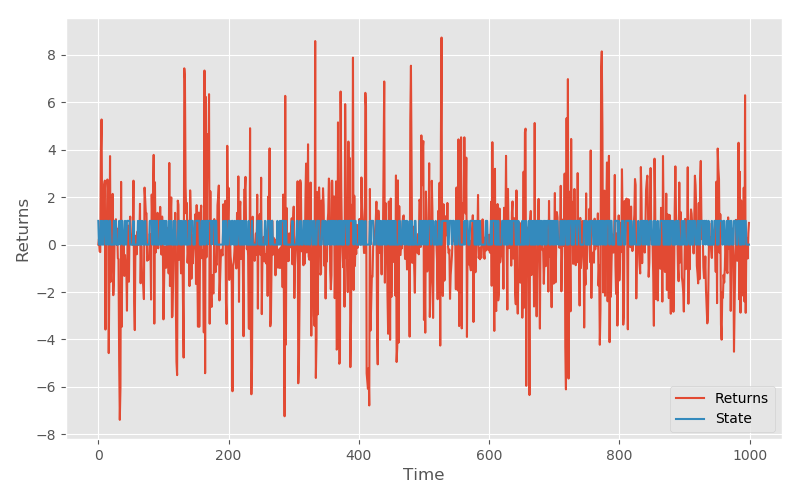
\includegraphics[scale = 0.45]{images/931a.png}
\end{minipage}
\hspace{0.5cm}
\begin{minipage}[b]{0.45\linewidth}
\centering
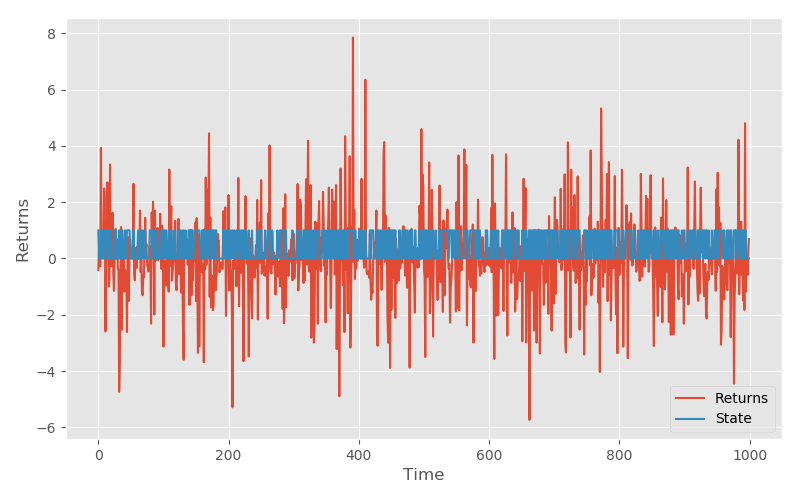
\includegraphics[scale = 0.45]{images/931b.png}
\end{minipage}
\begingroup
\subcaption*{Parameters: $\sigma_h = 2.0$, $\sigma_l = 0.5$, $\alpha_h = 0.5$, $\alpha_l = 0.9$, $p = 0.5$, seed = 12345.}
\endgroup
\end{figure}

The left panel of figure 2 below shows a state-switching Markov model with ARCH(1)-effects, whereas the right panel shows the same model but without ARCH-effects, but again built on the same random numbers. Both panels show that volatility has become more clustered, which is due to persistence in the state. The left panel shows more extreme returns, enforced by the ARCH-effect, where large returns follow large returns ($\alpha > 0$ in both states), and generally volatility varies within each volatility-state.
\begin{figure}[ht]
\centering
\captionsetup{justification=centering,margin=0.6cm}
\caption{State switching Markov models}
\begin{minipage}[b]{0.45\linewidth}
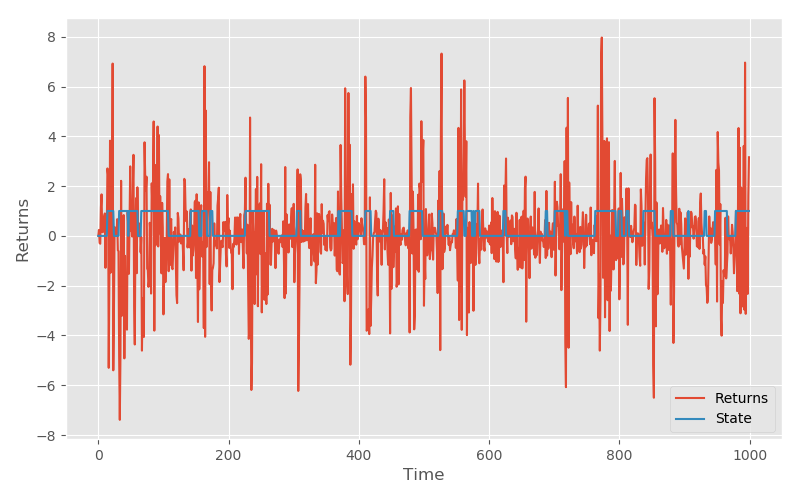
\includegraphics[scale = 0.45]{images/931c.png}
\end{minipage}
\hspace{0.5cm}
\begin{minipage}[b]{0.45\linewidth}
\centering
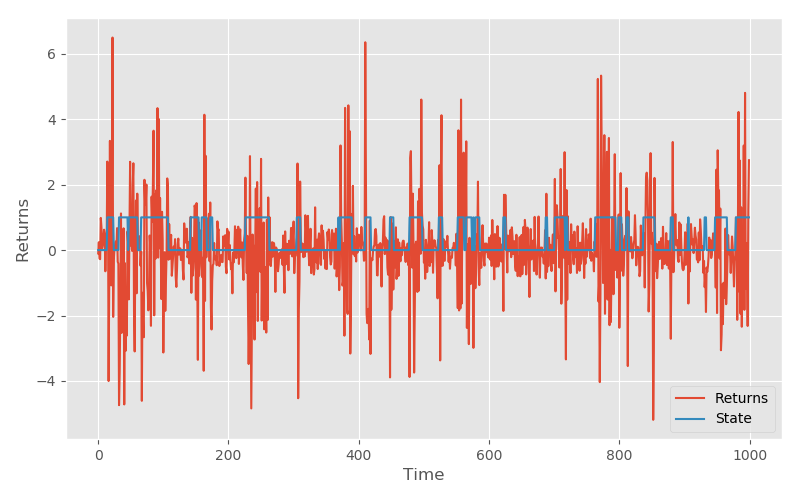
\includegraphics[scale = 0.45]{images/931d.png}
\end{minipage}
\begingroup
\subcaption*{Parameters: $\sigma_h = 2.0$, $\sigma_l = 0.5$, $\alpha_h = 0.5$, $\alpha_l = 0.9$, $p_{11} = 0.95$, $p_{22} = 0.90$, seed = 12345.}
\endgroup
\end{figure}

\subsection{Exercise 3.1}
When simulating the series, we assumed parameter values for $\theta = \lp \sigma_h, \sigma_l, \alpha_h, \alpha_l, p\rp$, which we now would like to estimate for some observed time series. We cannot observe the latent state variable $s_t$ and hence we cannot easily apply maximum likelihood.

\subsubsection{EM Algorithm for N-state switching SV Models}
As a solution to the problem above, we would derive the conditional maximum likelihood, take expectations, and maximise with respect to the parameters in the model, the so-called EM algorithm we treated in exercise 1.

In exercise 1, we had a state model, but no Markov-switching, which meant the smoothed probabilities had a closed-form solution and were thus easy to compute. Because the parameters are functions of the smoothed probabilities $p^*$, this scenario is ideal. In Markov-switching models the smoothed probabilities have no closed-form solution.

\subsubsection{Forward-backward algorithm}
Hamilton (1994) introduced a method for computing the smoothed probabilities, which he dubbed the forward-backward algorithm. The solution to the smoothed probabilities then look very similar:
\begin{align}
    p_t^* \lp j\rp = \frac{b_t^{rs}\lp j\rp a_t^{rs} \lp j\rp }{\sum_{k=1}^N b_t^{rs} a_t^{rs}\lp k\rp} & p_t\lp i, j\rp = \frac{b_t^{rs}\lp j\rp f\lp y_t\vert j\rp p_{ij} a_{t-1}^{rs} \lp i\rp }{a_{scale,t}\sum_{k=1}^N b_t^{rs} \lp k\rp a_t^{rs} \lp k\rp},
\end{align}
see lecture notes V for details.

With the smoothed probabilities computed, the parameter estimates follow, and estimation is concluded.

\subsection{1.1 Interpretation}
As introduced through the figures, the interpretation of the parameters are, that the volatility $\sigma_i^2$ determines the general level of volatility, and the ARCH-effect $\alpha_i$ determines the degree of variation of volatility within each regime.

\clearpage

\section{Exercise 4}
\renewcommand{\theequation}{4.\arabic{equation}}
\setcounter{equation}{0}

In this exercise we consider a two-state feedback volatility model, as given by:
\begin{align}
    y_t 
        &= \sigma_t z_t, \quad z_t \iid \nnn\lp 0, 1\rp \\
    \sigma_t^2 
        &= \begin{cases} \sigma_1^2, & s_t = 1 \\ \sigma_2^2, & s_t = 2 \end{cases},\\
    \pp\lp s_t = 1 \vert s_{1:t-1}, s_{1:t-1} \rp 
        &= p_1\lp y_{t-1}\rp \\
    \pp\lp s_t = 2 \vert s_{1:t-1}, s_{1:t-1} \rp 
        &= p_2\lp y_{t-1}\rp.
\end{align}

By assumption, $y_t$ is observed, $s_t$ is not.

An example of the probability $p_1\lp y_{t-1}\rp$ is:
\begin{align}
    p_1\lp y_{t-1}\rp = \frac{\exp\lc  a \lp y_{t-1} - b\rp \rc}{1 + \exp\lc a \lp y_{t-1} - b \rp \rc}\in ]0, 1[, \quad a > 0, b \in \rr.
\end{align}

The model parameters are then $\theta = \lp a, b\rp$.

\subsection{4.1}
We are asked to discuss ideas for $p_1\lp \cdot\rp$ and motivation for the idea of the model.

Alternative ideas for $p_1\lp y_t\rp$ requires that the probabilities are in $]0, 1[$ and that $p_1\lp y\rp + p_2\lp y\rp = 1$. As long as this is true, anything goes.

Disclaimer: The following is taken directly from class.

The specification above allows for different switching mechanisms (the same as used in logistic regressions for binary outcomes). An obvious alternative is the Gaussian CDF, which is used in the probit model for binary outcomes, $p_1\lp y_{t-1}\rp = \Phi\lp a y_{t-1}\rp$.

\subsection{4.2}
We are then asked to discuss simulation of the realisation of $s_t$ given $y_{t-1}$. To do this, we need to:
\begin{itemize}
    \item first need to set parameters $\theta = \lp a \in \rr_+, b\in \rr\rp$.
    \item Next, we decide some initial log-return $y[0] \in \rr$ (reasonable values would be somewhere between $[-3, 3]$, as most returns produced fall in this interval).
    \item Next, given the formula in (4.5) we decide $p_1\lp y_{t-1}\rp$.
    \item Finally, we simulate some random uniform number $u\sim U\lp 0, 1\rp$ to produce the state $s_t$.
\end{itemize}

The final point is, that if $p_1\lp y_{t-1}\rp < u$ then the state is $s_t = 1$, otherwise it is $s_t = 2$. From this we can simulate the time series of (4.1)-(4.4) as done in the left panel of figure 3 below (the right panel shows the state-switching model presented in the right panel of figure 1).

The result is very much like the regular model, but with more volatility.

\begin{figure}[ht]
\centering
\captionsetup{justification=centering,margin=0.6cm}
\caption{State-switching models}
\begin{minipage}[b]{0.45\linewidth}
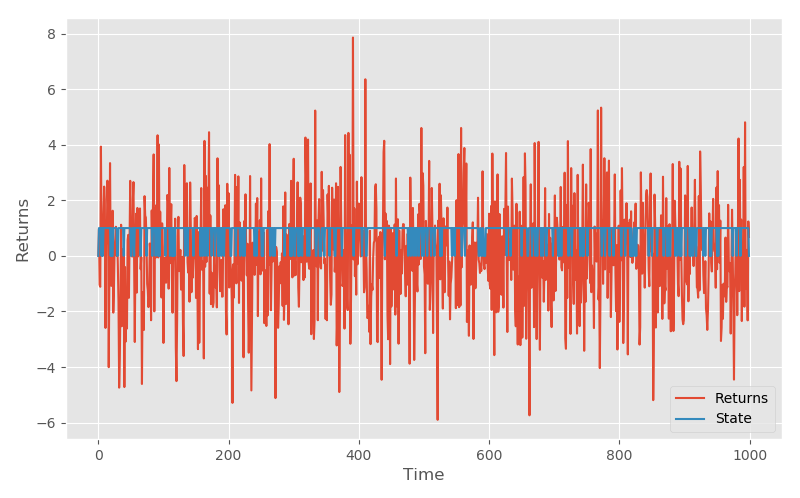
\includegraphics[scale = 0.45]{images/942.png}
\end{minipage}
\hspace{0.5cm}
\begin{minipage}[b]{0.45\linewidth}
\centering
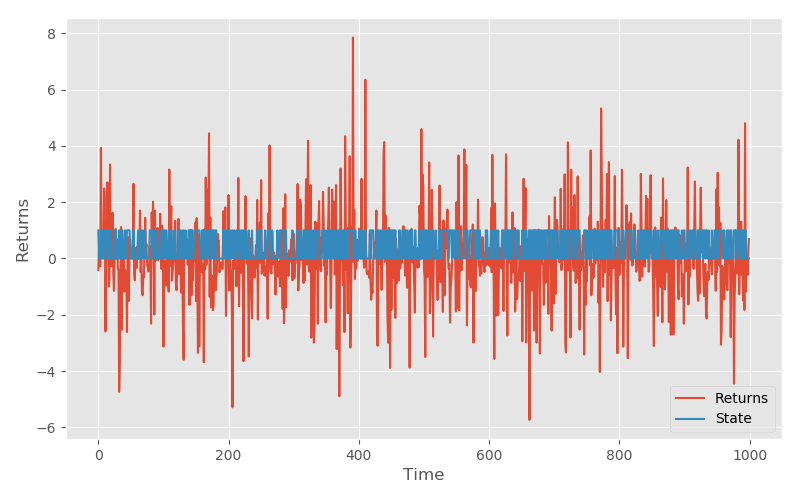
\includegraphics[scale = 0.45]{images/931b.png}
\end{minipage}
\begingroup
\subcaption*{Parameters: $\sigma_h = 2.0$, $\sigma_l = 0.5$, $\alpha_h = 0.5$, $\alpha_l = 0.9$, $p = 0.5$, seed = 12345.}
\endgroup
\end{figure}

\subsection{4.3}
Next, we are asked to derive the joint probability density function of $y_{1:T}, s_{1:T}$, $y_0$ given. We follow the same steps as previously:
\begin{align}
    f\lp y_{1:T}, s_{1:T}\rp 
        &= f\lp y_T \vert y_{1:T-1}, s_{1:T}\rp f\lp y_{1:T-1}, s_{1:T}\rp \notag \\
        &= f\lp y_T \vert y_{1:T-1}, s_{1:T}\rp f\lp s_T \vert y_{1:T-1}, s_{1:T-1}\rp f\lp y_{t:T-1}, s_{1:T-1}\rp.
\end{align}

From (4.6) we see that the final part of the RHS is equal to the LHS, reduced by the terminal period. Thus, by deduction we have that:
\begin{align}
    f\lp y_{1:T}, s_{1:T}\rp 
        &= \Pi_{t = 2}^T f\lp y_t \vert s_t\rp f\lp s_t\vert y_{t-1}\rp, \quad y_1\sim \text{given}.
\end{align}

Taking logs we have:
\begin{align}
    \ell_T\lp \theta\rp 
        &= \sum_{t=2}^T \log\lp f\lp y_t \vert s_t\rp \rp  + \log \lp \pp \lp s_t\vert y_{t-1}\rp\rp.
\end{align}

Consider the two density functions in turn:
\begin{align}
    f\lp y_t \vert s_t\rp = f\lp y_t \vert s_t = 1\rp^{\ii_1} f\lp y_t \vert s_t = 2\rp^{\ii_2}, \\
    f\lp s_t \vert y_{t-1}\rp = p_1\lp y_{t-1}\rp^{\ii_1} \lp 1 - p_1\lp y_{t-1}\rp\rp^{\ii_2}.
\end{align}

Substituting equations (4.9) and (4.10) into (4.8) gives the log-likelihood function:
\begin{align}
    \ell_T\lp \theta\rp = \sum_{t=2}^T \lc \ii_1\lb \log \lp f\lp y_t \vert s_t = 1\rp \rp + \log \lp p_1\lp y_{t-1}\rp \rp \rb + \ii_2\lb \log\lp f\lp y_t \vert s_t = 2\rp \rp + \log \lp 1 - p_1\lp y_{t-1}\rp \rp \rb \rc.
\end{align}

This is the furthest we can factorise the log likelihood function, and concludes exercise 4.3.

\subsection{4.4}
We are now asked to show that the E-step in the EM-algorithm yields:
\begin{align}
    \ell_{EM} = \sum_{t=2}^T \sum_{i = 1}^2 p_t^* \lp i\rp \lb \log p_i \lp y_{t-1}\rp + \log f_\theta\lp y_t\vert i\rp \rb,
\end{align}

where $p_t^*\lp i\rp = \pp \lp s_t = i\vert y_{1:T}\rp$, that is, we take the expectation with respect to all observed data $y_{1:T}$:
\begin{align}
    \ee\lb \ell_T \vert y_{1:T}\rb 
        &= \sum_{t=2}^T 
            \ee\lb \ii_1\vert y_{1:T} \rb 
            \lb 
                \log \lp f\lp y_t \vert s_t = 1\rp \rp + \log \lp p_1\lp y_{t-1}\rp \rp
            \rb
            \notag \\
            +&
            \ee\lb \ii_2\vert y_{1:T} \rb 
            \lb
                \log\lp f\lp y_t \vert s_t = 2\rp \rp + \log \lp 1 - p_1\lp y_{t-1}\rp \rp 
            \rb.
\end{align}

The conditional expectation to the indicator functions can be written as:
\begin{align}
    \ee\lb \ii_{\lc s_t = i \rc} \vert y_{1:T}\rb = \pp\lp s_t = i\vert y_{1:T}\rp, \quad i = 1, 2
\end{align}

such that equation (4.14) becomes:
\begin{align}
    \ee\lb \ell_T \vert y_{1:T}\rb 
        &= \sum_{t=2}^T 
            \pp\lp s_t = 1\vert y_{1:T}\rp
            \lb 
                \log \lp f\lp y_t \vert s_t = 1\rp \rp + \log \lp p_1\lp y_{t-1}\rp \rp
            \rb
            \notag \\
            +&
            \pp\lp s_t = 2\vert y_{1:T}\rp
            \lb
                \log\lp f\lp y_t \vert s_t = 2\rp \rp + \log \lp 1 - p_1\lp y_{t-1}\rp \rp 
            \rb
        \notag \\
        &=  \sum_{t=2}^T 
            \sum_{i = 1}^2
            \pp\lp s_t = i\vert y_{1:T}\rp
            \lb 
                \log \lp f\lp y_t \vert s_t = i\rp \rp + \log \lp p_i\lp y_{t-1}\rp \rp
            \rb
        \notag \\
        &=  \sum_{t=2}^T 
            \sum_{i = 1}^2
            p_t^*\lp i\rp 
            \lb 
                \log \lp p_i\lp y_{t-1}\rp \rp +
                \log \lp f\lp y_t \vert i\rp \rp
            \rb
\end{align}

which is the expression we wanted to show, and where we have used that $p_2 \lp y_{t-1}\rp = 1 - p_1\lp y_{t-1}\rp$ by definition.

\subsection{4.5}
We are now told to consider that:
\begin{align}
    p_t^*\lp i\rp  = \pp\lp s_t = i\vert y_{1:T}\rp = \pp\lp s_t = i \vert y_{t-1}, y_t\rp,
\end{align}

which we asked to use to show that:
\begin{align}
    p_t^*\lp i \rp = \frac{p_i\lp y_{t-1}\rp f\lp y_t \vert i\rp }{\sum_{t=1}^2p_i\lp y_{t-1}\rp f\lp y_t\vert i\rp}.
\end{align}

First, we have that $\pp\lp s_t = i \vert y_{t-1}, y_t\rp = f\lp s_t = i\vert y_{t-1}, y_t\rp$. Further recall from (4.3) and (4.4) that $p_i \lp y_{t-1}\rp = \pp\lp s_t = i \vert s_{1:t-1}, y_{1:t-1}\rp = \pp\lp s_t = i \vert y_{t-1}\rp$. This can be used to derive the following:
\begin{align}
    p_t^*\lp i\rp = f\lp s_t = i\vert y_{t-1}, y_t\rp 
        &= \frac{f\lp s_t = i, y_t, y_{t-1}\rp}{f\lp y_t, y_{t-1}\rp} \notag \\
        &= \frac{f\lp y_t \vert s_t = i, y_{t-1}\rp f\lp s_t = i \vert y_{t-1}\rp f\lp y_{t-1}\rp }{f\lp y_t, y_{t-1}, s_t = 1\rp + f\lp y_t, y_{t-1}, s_t = 2\rp} \notag \\
        &= \frac{p_i\lp y_{t-1}\rp f\lp y_t \vert s_t = i\rp f\lp y_{t-1}\rp}{\lp f\lp y_t \vert s_t = 1\rp f\lp s_t = 1\vert y_{t-1}\rp + f\lp y_t \vert s_t = 2\rp f\lp s_t = 2 \vert y_{t-1}\rp \rp f\lp y_{t-1}\rp} \notag \\
        &= \frac{p_i\lp y_{t-1}\rp f\lp y_t \vert s_t = i\rp}{\sum_{i=1}^2 p_i\lp y_{t-1}\rp f\lp y_t \vert s_t = i \rp},
\end{align}

where the second equality follows from the law of total probability.

\subsection{4.6}
Finally, we are asked to find $\hat{\tilde \sigma_1^2}$ in terms of $p_t^*\lp \cdot \rp$ and $y_t$, $t = 1, \dots, T$.

We note that:
\begin{align}
    \log \lp f\lp y_t \vert 1\rp\rp = - \frac{1}{2}\lp \log \lp 2 \pi\rp + \log \lp \tilde \sigma_1^2 \rp + \frac{y_t^2}{\tilde \sigma_t^2}\rp.
\end{align}

To do this, we maximise (4.12) with respect to $\tilde \sigma_1^2$ by differentiation, i.e.:
\begin{align}
    \frac{\partial \ell_{EM}}{\partial \sigma_1^2}
        &= \sum_{t=2}^T p_t^*\lp 1\rp \lp \frac{1}{\tilde \sigma_1^2} - \frac{y_t^2}{\tilde \sigma_1^4}\rp 
        = \sum_{t=2}^T p_t^*\lp 1\rp \lp 1 - \frac{y_t^2}{\tilde \sigma_1^2}\rp\frac{1}{\tilde \sigma_1^2} 
        = 0 \notag \\
    \LL \tilde \sigma_1^2 \sum_{t=2}^T p_t^*\lp 1\rp &= \sum_{t=2}^T p_t^*\lp 1\rp y_t^2 \notag \\
    \LL \tilde \sigma_1^2 
    &= \frac{\sum_{t=2}^T p_t^*\lp 1\rp y_t^2}{\sum_{t=2}^T p_t^*\lp 1\rp}.
\end{align}

This result is quite intuitive, in that it sums all the volatility that occurs when the state is 1 and averages out over all the periods when the state is 1. That is, we are taking an average of the volatility observed in a period we believe to be of state 1, and defining this volatility as the state-1 volatility. Very intuitive and very elegant.

\clearpage

\section{Exercise 5}
This was not covered in class.

\end{document}